\documentclass[11pt,a4paper]{article}
\usepackage{a4wide,url,enumitem,graphicx}
\usepackage[utf8]{inputenc}
\usepackage[main=english,russian]{babel}
\usepackage{csquotes}

\setlist{noitemsep}
\parindent0pt
\parskip4pt
\setcounter{tocdepth}{2}

\title{Research Seminar "Sustainability, Environment, Management". Seminar
  Notes}

\author{Hans-Gert Gr\"abe}

\date{Winter Term 2021/22}

\begin{document}
\maketitle
\tableofcontents
\newpage

\section{About the Course}

The course consists of
\begin{itemize}
\item the lecture "Modelling Sustainable Systems and Semantic Web",
\item the Research Seminar "Sustainability, Environment, Management" and
\item optionally a practical online lab "Introduction to TRIZ". 
\end{itemize}

In this course, the focus is on the prerequisites and conditions associated
with sharpening the meaning of notions in concrete contexts. Technical issues
of the Semantic Web\footnote{See
  \url{https://www.semantic-web-grundlagen.de}.} will be addressed only
marginally, as we assume that sufficient materials exist on the web to learn
more about such concepts to the extent required for practical purposes.

The course is designed as an \textbf{interdisciplinary academic course}.

\textbf{Interdisciplinary} means that colleagues from different areas are
involved – Sabine Lautenschläger (IIRM), Ken Pierre Kleemann (philosophy),
Ralf Laue, Kristin Kutzler and Hans-Gert Gräbe (computer science).

\textbf{Academic} means that we want to work with each other and with the
students – especially in the seminar – at equal level. It is about rational
argumentation on a scientific level, i.e. we count for \emph{arguments} and not
apodictic truths.

All materials and seminar reports that can be made publicly available, are be
published in the github repository
\url{https://github.com/wumm-project/Seminar-W21}.

\subsection{Modelling Sustainable Systems and Semantic Web}

The Semantic Web extends the Web in order to make data easier to exchange
between computers and make it easier to use; for example, the term "Bremen" in
a web document can be supplemented with information as to whether it refers to
a ship with that name, a family name or the town "Bremen". This additional
information makes information explicit in otherwise unstructured data. To add
such information in a formalised way Semantic Web standards for the
publication and use of machine-readable data (especially RDF) are applied.

This is a \emph{very technical view} that does not take into account,
\emph{why} these distinctions are relevant at all. In this more general sense
\textbf{Semantic Web Technologies are concerned with the sharpening of the
  meaning of concepts in particular contexts}.

These challenges are part of another core informatics competence – the ability
to elicit corresponding requirement complexes within the framework of
\emph{Requirements Engineering}, to structure and finally to model them.

The \textbf{focus of the lecture} is on the connection of these two complexes
of competences, whereby it is assumed that students in computer science
already have a basic knowledge of both areas. A special focus is on the
\emph{resolution of contradictory requirement situations} as the core of
systematic innovation methodologies such as TRIZ.

\subsection{Aim and Methodology of the Seminar}

The concept of a \emph{system} plays a prominent role in computer science when
it comes to database systems, software systems, hardware systems, accounting
systems, access systems, etc.  In general, computer science is regarded by a
majority as the "science of the \emph{systematic} representation, storage,
processing and transmission of information, especially their automatic
processing using digital computers" (German Wikipedia).  Also certain relevant
professions such as the \emph{system architect} are in high esteem by IT
users.

However, the significance of the concept of system extends far beyond the
field of computer science -- it is fundamental for all engineering sciences
and as \emph{Systems Engineering} with the ISO/IEC/IEEE-15288 standard
"Systems and Software Engineering", it is also the subject of international
standardisation processes.  Even more, the concept of systems also plays an
important role in the description of complex natural and cultural processes --
for instance in the concept of an \emph{ecosystem}.

While classical TRIZ focuses strongly on instrumentally feasible engineering
solutions, Systems Engineering "is an interdisciplinary field of engineering
and engineering management that focuses on how to design, integrate, and
manage complex systems over their life cycles. At its core, systems
engineering utilizes systems thinking principles to organize this body of
knowledge. The individual outcome of such efforts, an engineered system, can
be defined as a combination of components that work in synergy to collectively
perform a useful function." (English Wikipedia). 

Earlier in this seminar, we had already studied more intensively different
system concepts and, in particular, examined their application in complex
socio-ecological, socio-economic and socio-technical contexts, see
\cite{GraebeKleemann}. We observed that the central concepts of \emph{transition
  management} and \emph{activity management} addressed two different
perspectives on structural change processes. In the transition management
approach, the structural-transitional challenges are in the foreground, the
activity management approach studies the implementation of structural changes
via the actions and co-actions of actors and stakeholders.

In both approaches, however, the focus was on a holistic-structural and
analytical view of a \emph{decision preparation} rather than on practical
procedural management approaches of \emph{decision-making} and decision
implementation in complex and contradictory real-world situations.

The WUMM project\footnote{See \url{www.leipzig-netz.de/index.php/WUMM}. WUMM
  stands in German for \emph{Widersprüche und Managementmethoden}
  (Contradictions and Management Methods).} aims at a better understanding of
such management processes. Our starting point is TRIZ as a systematic
innovation methodology derived from engineering experience in contradictory
requirement situations. With the field of "Business TRIZ", which has been
unfolding for about 20 years, a transfer of experience is being actively
promoted, embedded in older management cultures and theories.  A better
understanding of such approaches to management issues and their connection to
systemic concepts and approaches was in the focus of our seminar last
semester.

In the seminar, we want to learn more about such modern management appoaches
in which \emph{common conceptualisations} and \emph{consensus-oriented
  decision-making processes} are central and of crucial importance for the
success and ways of formation and consolidation of new systemic structures.
We are particularly interested in the connection between the dialectical
resolution of contradictory requirement situations in the sense of TRIZ
methodology and the emergence of common conceptual and notational worlds as a
result of the application of suitable semantic web technologies.  A special
emphasis will be put on the work of the \emph{Methodological School of
  Management} around G.P. Shchedrovitsky \cite{MSM}.

The seminar is a research seminar in which we jointly explore different
aspects of co-operative action in different management concepts.  With this
seminar, we are approaching a topic that is new to us, which offers the
opportunity to participate in a joint academic explorative process on a basis
of equals. 

\section{On the Notion of a System}

\subsection{Once more about the Goal of the Seminar}

Systematic innovation methodologies such as TRIZ are essentially based on a
better understanding of the development dynamics of corresponding (technical
and non-technical) \emph{systems}.  The results are rooted in engineering
experience from structured processes of planning, implementation and operation
of technical systems. Increasingly, cooperative interdisciplinary
collaboration matters rather than the one brilliant mind that commands
thousand hands. The \emph{socio-technical character} of contradictions is
thereby intensified and opens up new dimensions of contradiction management.

Today, managers face similar challenges when it comes to placing
decision-making processes on a systematic basis, aligning the processes under
control with long term goals, and also achieving the targeted goal corridors.
It turns out that many engineering experiences on structured procedures in
contradictory requirement situations can be transferred to this area, which
has been investigated within the topic "TRIZ and Business" for 20 years.

Nevertheless, experiences and approaches to theories of systemic concepts are
based more broadly and also have much longer historical traditions.  \emph{In
  the seminar}, we want to study such concepts more closely, with special
emphasis on cooperative approaches in interdisciplinary contexts.

\subsection{What is a System?}

Operation and use of technical systems is a central element of today world
changing human practices. For this purpose planned and coordinated action
along a division of labour is necessary, because exploiting the benefit of a
system requires its operation. Conversely, it makes little sense to operate a
system that is not being used. Closely related to this distinction between
definition and call of a function, well known from computer science, is the
distinction between design time and runtime, that is even more important in
the real-world use of technical systems – during design time, the principal
cooperative interaction is planned, during the runtime the plan is executed.
For technical systems one has to distinguish the description, interpersonally
communicated as justified expectations, and the results of operation,
interpersonally communicated as practical experience.

Most definitions grasp the term \emph{system} as a delimited set of
interacting components, whereby the interaction of the components gives rise
to a unified whole, which realises an emergent function and is thus more than
the sum of its parts.
\begin{quote}
  A \emph{system} (lat. greek "system", "composed", a whole consisting of
  parts; connection) is a set of elements that are interconnected and interact
  with each other, forming a unified whole that possesses properties that are
  not already contained in the constituent elements considered individually.
  \cite{Petrov2020}

  A \emph{system} is a set of elements that are in relationship and connection
  with each other and that constitute a well defined unity, an integrity. The
  necessity of the use of the term "system" occurs when it is required to
  emphasize that something is large, complex, immediately not wholly
  comprehensible, but at the same time a unified whole. Unlike the notions
  "set" or "aggregate", the concept of a system emphasizes the ordering, the
  integrity, the regularity of construction, functioning and development.
  \cite{TOP}

  Systems Engineering "is an interdisciplinary field of engineering and
  engineering management that focuses on how to design, integrate, and manage
  complex systems over their life cycles. At its core, systems engineering
  utilizes systems thinking principles to organize this body of knowledge. The
  individual outcome of such efforts, an engineered system, can be defined as
  a combination of components that work in synergy to collectively perform a
  useful function." (English Wikipedia).
\end{quote}
The second definition also points to the purpose of systemic delimitations --
it is about making complex relationships accessible to description by reducing
them to essentials.

In all these definitions, the \emph{structuredness} and thus
\emph{decomposability} of the system in the analytic dimension is emphasised
on the one hand, and the \emph{interdependence} and thus
\emph{indecomposability} in the execution dimension on the other. This
corresponds to the practical experience of the engineer when she assembles a
system from individual components -- the system is only viable when it is
assembled. In the assembled system in addition to the components, the
\emph{connecting elements} also play an important role.  They mediate the
\emph{flow of energy, material and information} that is required for the
operation of each component. In component software \cite{Szyperski2002}, with
\emph{deployment}, \emph{installation} and \emph{configuration} three stages
of preparing components for their operation in a systemic context are
distinguished, and this preparation for operation is often considered as a
separate state -- for example, as \emph{maintenance mode} different from the
\emph{operation mode}.

The aspect of operating a system did not play a role in the first two
definitions.  Only here, however, the dialectical interrelationship between
decomposability and indecomposability comes to light: Viable components
deliver processual services in \emph{guaranteed} quantity and quality during
operation, if the \emph{external operational conditions} are guaranteed.
These processual services of the components in combination form the emergent
function of the overall system. The self-similarity of the concept is obvious:
components themselves have an inner life that can be described systemically,
but which is largely abstracted from at the level of the overall system. The
component enters the description of the dynamics of the overall system only as
Black Box with a precise specification.  This specification is divided into
input and output interfaces.  The former describe the necessary operating
conditions, the latter the performance parameters of the respective component.

In \cite{Graebe-mts} the system concept is identified as descriptional
focusing to make real-world phenomena accessible for a description by
reduction to the essentials.  Such a reduction focuses on the following three
dimensions:
\begin{itemize}
\item[(1)] Outer demarcation of the system against an \emph{environment},
  reduction of these relationships to input/output relationships and
  guaranteed throughput.
\item[(2)] Inner demarcation of the system by combining subareas to
  \emph{components}, whose functioning is reduced to “behavioural control” via
  input/output relations.
\item[(3)] Reduction of the relations in the system itself to “causally
  essential” relationships.
\end{itemize}
Further, it is stated that such a reductive description (explicitly or
implicitly) exploits output from prior life:
\begin{itemize}
\item[(1)] An at least vague idea about the (working) input/output services of
  the environment.
\item[(2)] A clear idea of the inner workings of the components (beyond the
  pure specification).
\item[(3)] An at least vague idea about causalities in the system itself, that
  precedes the detailed modelling.
\end{itemize}

\subsection{Systems, Components and Reuse}

One important aspect, especially of technical systems, has not yet been taken
into account in the considerations so far: the aspect of reuse. Reuse plays a
central role in computer science -- copy/paste of code, outsourcing of
repetitive pieces of code in function definitions, grouping of related
function definitions in pre-compiled libraries, etc. This in no way exhausts
possible forms of reuse, not to mention higher forms of reuse such as design,
patterns or frameworks. Szyperski discusses in \cite[ch. 8]{Szyperski2002}
aspects of the relationship between goals and forms of reuse.

Hence in addition to the description and operation, for technical systems the
aspect of reuse plays an important role. However, this does not apply, at
least on the artifact level, to larger technical systems – these are unique
specimen, even though assembled using standardised components. Also the
majority of computer scientists is concerned with the creation of such unique
specimens, because the IT systems that control such plants are also unique.

Computer science has long struggled with a form of reuse that is widespread in
developed engineering sciences and ultimately turned the manufacturing of
tools and products from an art first to a craft and later to an industrial
process -- the \emph{use of components produced by third parties} (components
off the shelf).

Thus, after the analytical and operational dimension of systems and
components, the \emph{production by independent third parties} and hence the
technical-economic interrelationships of an industrial mode of production
based on the division of labour move into the focus of attention.

In such a context, the concept of a technical system is fourfold overloaded.
A technical systems can be considered
\begin{itemize}
\item [1.] as a real-world unique specimen (e.g. as a product or a service),
\item [2.] as a description of this real-world unique specimen (e.g. in the
  form of a special product configuration)
\end{itemize}
and for components produced in larger quantities also
\begin{itemize}
\item [3.] as description of the design of the system template (product
  design) and
\item [4.] as description and operation of the delivery and operating
  structures of the real-world unique specimens of this system produced
  according to this template (as production, quality assurance, delivery,
  operational and maintenance plans).
\end{itemize}
The concept of a technical system thus has also in this context a clearly
epistemic function of (functional) ``reduction to the essential''. To Einstein
the recommendation is attributed ``to make things as simple as possible but
not simpler''. The TRIZ \emph{law of completeness of a system} expresses
exactly this thought, however, not as a \emph{law}, but as an engineering
\emph{modeling directive}. The apparent ``law'' of the observed dynamics
therefore essentially addresses \emph{reasonable human action}.

In an approach of ``reduction to the essential'' and ``guaranteed
specification-compliant operation'' human practices are inherently built in,
since only in such a context the terms ``essential'', ``guarantee'' and
``operation'' can be filled with sense in a meaningful way. These essential
terms from the socially determined practical relationship of people are deeply
rooted in the concept generation processes of descriptions of special
technical systems and find their ``natural'' continuation in the special
social settings of a legally constituted societal system.

\subsection{Socio-technical Systems}

The last considerations already embed the concept of system in social
practices of cooperatively acting people. This embedding is also present in
TRIZ system definitions, when the emergent function realised by the system is
considered as \emph{main useful function} MUF and linked to a \emph{purpose},
why this (technical) system exists or was designed or redesigned in this way.
This \emph{aspect of purposefulness} (Zweckmäßigkeit) plays only a subordinate
role for "natural" systems, namely for socio-ecological systems, since in this
context in most cases the "purposefulness" comes up against hard limits or
causes massive problems or has even already caused them. Nevertheless, this
\emph{orientation on purposes} is another throughput parameter (e.g. as
monetary throughput) from a social environment relevant for the inner dynamics
of a system.  It can ultimately be subsumed under the \emph{throughput of
  information} if a sufficiently viable concept of information is taken as a
basis. 

This purposefulness transforms the totality of technical systems into an
interconnected \emph{world of techical systems} full of preconditions and
conditionalities, which opens up a fourth dimension of the concept of system,
to secure stable operating conditions of the systems themselves.

The self-similarity of the systems concept provides a solution for this
challenge -- consider systems as components and the relations of
purposefulness as interdependencies, delineate larger socio-technical systemic
units, develop appropriate forms of description and operation. The
transformation towards a sustainable mode of production and living that is on
the agenda just requires a big step forward in this direction.  This is one of
the objectives of management and hence in the primary focus of our seminar.
However, socio-technical systems are, in addition to technical restrictions,
charged with the contradictory expectations and interests of concrete people
and groups of people.

Ian Sommerville \cite{Sommerville2015} elaborates a number of challenges in
this regard. He also starts with the concept of a goal-centered system.
\begin{quote}
  A \emph{system} is a meaningful set of interconnected components that work
  together to achieve a specific goal.  \cite{Sommerville2015}
\end{quote}
Right after he develops a distinction between technical and socio-technical
systems:

\paragraph{Technical computer-based systems}
are systems that contain hardware and software components, but not procedures
and processes. ... Individuals and organisations use technical systems for
specific purposes, but knowledge of that purpose is not part of the system.
For example, the word processor I use does not know that I am using it to
write a book.

\paragraph{Socio-technical systems}
contain one or more technical systems, but beyond that -- and this is crucial
-- the knowledge of how the system should be used to achieve a broader
purpose.  This means that these systems have \emph{defined work processes},
\emph{human operators} as integral part of the system, are \emph{governed by
  organisational policies} and are \emph{affected by external constraints}
such as national laws and regulations.

Essential characteristics of socio-technical systems:
\begin{enumerate}
\item They have special properties that affect the system as a whole, and are
  not related to individual parts of the system. These special properties
  depend on the system components and the relationships between them. Because
  of this complexity, the system-specific properties can only be evaluated
  when the system is composed.
\item They are often not deterministic. The behaviour of the system depends on
  the human operators and on other people who do not always react in the same
  way. Also, the operation of the system can change the system itself.
\item The extent to which the system supports organisational goals depends not
  only on the system itself. It also depends on the \emph{stability of the
    goals}, the relationships and \emph{conflicts between organisational
    goals}, and how people in the organisation \emph{interpret those goals}.
\end{enumerate}

In this context, there is a clear shift on the scale of controllability from
direct control by external human operators to indirect control and movement
according to intrinsic laws, which is even more prevalent in
\textbf{socio-economic systems} with a large number of stakeholders or even
\textbf{socio-ecological systems}.

\subsection{Shchedrovitsky on Systems Analysis}

The system concept thus serves to delimit a part of the complex, all-connected
world (hereafter \emph{reality}) in order to make this part accessible for
description. However, this human activity, which Georgi Shchedrovitsky (a
Russian Philosopher and the head of the \emph{Methodological School of
  Management}) refers to as \emph{mental activity} \cite[p. 47]{MSM}, is
itself part of that reality and thus also of practical relevance. Real-world
processes are thereby charged with description forms. Thus in systems these
two dimensions -- description and operation -- must therefore be
distinguished. Charging a system with a description form is what Engels'
calls, in reference to Kant's \emph{thing in itself}, the transformation of
the \emph{thing in itself} into a \emph{thing for us}.

Shchedrovitsky \cite[p. 80 ff.]{MSM} conceptualises this process in two
different concepts of system \cite[pp. 89 and 98]{MSM} as process of breaking
down the system into parts (components), charging the components with
description forms and then reassembling the components thus charged into a
whole.  The result is a \emph{new} system in the sense that it is the old one
but charged with a description form.  In this way, the \emph{structural
  organisation} of a system can be grasped.

The real world and thus also systems develop and change over time. In order to
understand the \emph{development of a system}, its \emph{processual
  organisation} must be examined.  Shchedrovitsky emphasises that the
development of a system can \emph{never} be described in its disassembled
form, since disassembly destroys the systemic coherence. An aeroplane
disassembled into its individual parts cannot fly, only an assembled one. We
are dealing here with a fundamental epistemic contradiction.

For details we refer to \cite{MSM}.

\subsection{Theory of Dynamical Systems}

\subsubsection{The Approach}

The processual dimension of systems can be investigated with the mathematical
tools of the Theory of Dynamical Systems if the processes can be modelled as
equations of motion in phase space.

The Theory of Dynamical Systems as a branch of mathematics investigates the
dynamics of structurally defined and modelled systems. Attributes which are
essential for the description of the system are combined into a \emph{phase
  space} and the changes in the attribute values are described as
\emph{equations of motion} by differential equations. If only temporal changes
are considered, this leads to systems of \emph{Ordinary Differential
  Equations} (ODE), complex spatio-temporal changes lead to Partial
Differential Equations. We restrict ourselves to the first case, i.e. purely
temporal structural changes.

In the simplest case, such as the pendulum or the movement of two bodies in a
homogeneous gravitaional field, a \emph{trajectory} can be calculated from the
equations of motion.

Examples:
\begin{itemize}
\item Pendulum: \url{https://en.wikipedia.org/wiki/Pendulum_(mechanics)}
\item Two body problem: \url{https://en.wikipedia.org/wiki/Two-body_problem}
\end{itemize}

\subsubsection{Model and Reality}

However, the solution of this equations only describes the motion $m(t)$ in
the model. Good modelling is characterised by the fact that the real movement
$f(t)$ and the movement $m(t)$ according to the model differ only
insignificantly $r(t)=f(t)-m(t)$ in practically relevant parameter ranges (the
\emph{context of observation}). This can only be verified empirically through
experiments that are to be planned more or less precisely, since reality is
only accessible empirically.

Particularly interesting are modellings in which the residual $r(t)$ decreases
"by itself". Such systems strive towards an equilibrium, which structure can
be derived from the model.

\subsubsection{How Chaotic can Trajectories be?} 

Examples: 
\begin{itemize}
\item Double Pendulum, \url{https://en.wikipedia.org/wiki/Double_pendulum}
\item Magnetic pendulum with three attracting magnets,
\item 3-body model: \url{https://en.wikipedia.org/wiki/Three-body_problem}
\end{itemize}

We see that there is apparent stability for a long time, but in phase space
there are certain \emph{areas of instability} in which (exactly calculable!)
trajectories passing through points in phase space that are close to each
other strongly diverge. Such locations are called \emph{bifurcations}.  Often
there is a single phase parameter that makes this bifurcation particularly
clear. Such a bifurcation on a one-dimensional scale is also called a
\emph{tipping point}.

Not everything that looks like chaos has to be chaotic:\\
\url{https://i.redd.it/zr7tet9mdfl01.gif}

\subsubsection{Attractors}

How complicated can an equilibrium position be? 

Examples: 
\begin{itemize}
\item Pendulum,
\item pendulum with three attracting magnets,
\item pendulum with one repelling magnet.
\end{itemize}

Limit cycles: \url{https://en.wikipedia.org/wiki/Limit_cycle}

When the body is on the limit cycle, it remains there, i.e. the limit cycle is
a \emph{stable solution} of the equations of motion of the system, called
\textbf{steady-state equilibrium}.
    
In many cases the real movement $f(t)$ in time is \emph{attracted} by that
limit cycle, i.e. $f(t)$ can be decomposed into $f(t)=l(t)+r(t)$ with $l(t)$
the projection on the limit cycle and $r(t)$ a (small) orthogonal deviation.
In this way, it is often possible to simplify complicated models.

An attractor is a specific steady-state equilibrium with just this attracting
property.

More precisely: Let $f(t,a)$ be a function which specifies the dynamics of the
system with starting point $f(0,a)=a$. An \textbf{attractor} is a subset $A$
of the phase space characterized by the following three conditions:
\begin{itemize}
\item $A$ is forward invariant under $f$: if $a$ is an element of $A$ then so
  is $f(t,a)$, for all $t > 0$.  
\item There exists a neighborhood of $A$, called the basin of attraction for
  $A$ and denoted $B(A)$, which consists of all points $b$ that "enter $A$ in
  the limit $t\to\infty$".
\item There is no proper (non-empty) subset of $A$ having the first two
  properties.
\end{itemize}

Attractor as stable solution of the corresponding system of ODE\\
\url{https://en.wikipedia.org/wiki/Attractor}

\paragraph{On the importance of "stable" cyclical processes in nature.}
We are able to perceive such \emph{approximately} repeating patterns in
natural processes (i.e. attractors), i.e.  perform such a reduction also
independently of mathematical abilities.

For given (deterministic) equations of motion one can compute the geometry of
such an attractor as \emph{global deterministic} invariant of the equations of
motion.

\paragraph{How Complicated can an Attractor be?}
\begin{itemize}
\item \url{https://en.wikipedia.org/wiki/Attractor}
\item \url{https://en.wikipedia.org/wiki/Lorenz_system}
\item \url{https://de.wikipedia.org/wiki/Lorenz-Attraktor}
\item Attention, with the numerical methods used there for visualisation it is
  difficult to distinguish whether they are calculating a chaotic trajectory
  or really the attractor, which is a \emph{global} artefact.
\item "Almost all initial points will tend to an invariant set – the Lorenz
  attractor – a strange attractor, a fractal, and a self-excited attractor"
  (Wikipedia)
\end{itemize}

\subsubsection{Dissipative Systems}

Closed and Open Systems. Previous investigations were directed towards the
inner dynamics of an autonomous, i.e. closed system.

Importance of a (stable) throughput of energy, matter and information for the
inner structure formation in systems.

\begin{itemize}
\item Self-organisation in dissipative structures
  \begin{itemize}
  \item \url{https://en.wikipedia.org/wiki/Rayleigh-Bénard_convection}
  \item \url{https://en.wikipedia.org/wiki/Belousov-Zhabotinsky_reaction}
  \end{itemize}
\item Dissipative systems
  \url{https://en.wikipedia.org/wiki/Dissipative_system} 
\item Life on Earth as a dissipative system.
\end{itemize}

\section{Systems, Organisations, Management (Gräbe)}

\subsection{Organisations as Systems}

Systematic innovation methodologies such as TRIZ are essentially based on a
better understanding of the development dynamics of corresponding (technical
and non-technical) \emph{systems}.  The results are rooted in engineering and
managerial experience from structured processes of planning, implementation
and operation of such systems. Increasingly, cooperative interdisciplinary
collaboration matters rather than the one brilliant mind that commands
thousand hands. The \emph{socio-technical character} of contradictions is
thereby intensified and opens up new dimensions of contradiction management.

This seminar topic aims to shed more light on the connection between the
concepts of system and (social) organisation. \textbf{Social organisations}
such as companies, associations, projects, unions, parties, governments,
states ... are undoubtedly theoretically delimitable and practically delimited
parts of reality with outwardly (and inwardly) directed goals and purposes
whose internal structure and dynamics are driven by an external throughput of
energy, material and information, and which can therefore be studied from a
systemic perspective.

The external throughput of energy, material and information is usually not in
the focus of consideration, as these throughputs are already mentally charged
in language form in a \textbf{more complex social context} and in the form of
interests, needs, monetary flows and power relations. Nevertheless, a systemic
structure is clearly recognisable, which is to be worked out in various
theoretical approaches that we will look at in more detail. In particular, the
concepts of \emph{action space} and \emph{cooperative action} in such spaces
will be conceptualised in more detail.

\subsection{Leadership and Management}

\emph{Management} is an essential form of influencing the dynamics and
development of organisations. Shchedrovitsky emphasises that one can only
manage something that is in motion\footnote{"Management is only possible if
  the object we manage is in motion, self-propulsion. Management is the use of
  this self-propulsion by managers for their own purposes." \cite[p. 28]{MSM}}
and that there is no need for management if there are no problems.

In the previous semester, we had already considered the topic by studying
different theoretical approaches to management.  Most of them assumed a
manager as a single leader and developed approaches and patterns of how
persons in such a \emph{role} can develop leadership in achieving given goals.
If we project such approaches onto a systemic concept of development in
contradictions, there seems to be a recurring central contradiction between
the goals of the organisation and the goals and interests of the people
involved in realising them.

However, such leadership principles have been under massive pressure for at
least 20 years, as they have only limited effect in modern contexts of action
in interdisciplinary teams. Even more, they presuppose the authorised
individual leader who combines management and leadership in one person. In
multi-stakeholder contexts such as socio-cultural or socio-ecological systems,
even this prerequisite is not given.

In this context, Shchedrovitsky clearly distinguishes between the notions of
\emph{management} and \emph{leadership} \cite[p. 27-30]{MSM} and shows to what
extent a new principal is confronted with contradictory challenges of both
concepts.

\subsection{Systemic Management Basics}

In the further course of the seminar we want to discuss the systemic
development of social organisations in the unity and difference of
\emph{planned action} and \emph{experienced results} in the light of different
theoretical approaches.

This requires a concept of \emph{action planning}, based on a \emph{conceptual
  understanding} of the process landscape within and around the organisation
in an appropriate explicit form of description and \emph{intelligible
  operational actions}.

The formulated intelligible actions -- the \emph{plan} -- is in
\emph{contradictory tension} with the processes actually taking place: On the
one hand, it has a controlling effect on these practices, on the other hand,
those practices partially resist this control.

This difference must be fed back to the planning process as an
\emph{evaluation of experienced results} in order to keep also the divergence
between plan and reality under control.

Relating planning and experience dimension is only possible on a language
level and requires a \emph{system of notions} to accompany the practical
real-world development by a discursive process (as \emph{practice of thinking}
in the unity and difference of \emph{pure thought} and \emph{mental activity}
as explained in \cite[p. 33-51]{MSM}).

This system of concepts is more stable than the real-world practices, but it
is not static -- it develops together with the practices.
\textbf{\emph{World} is \emph{reality for us} and thus reality in the process
  of conceptual grasping.}

These basic considerations are about \emph{processes} and \emph{procedures}
within an \emph{organisation}.

\subsection{Organisations}

What is an organisation? Wikipedia distinguises between formal aud informal
organisations. 

\paragraph{Formal organisations.}
\begin{quote}
  An organisation that is established as a \emph{means for achieving defined
    objectives} has been referred to as a formal organisation. Its design
  specifies how \emph{goals are subdivided and reflected} in subdivisions of
  the organisation. Divisions, departments, sections, positions, jobs, and
  tasks make up this work structure. Thus, the formal organisation is expected
  to \emph{behave impersonally} in regard to relationships with clients or
  with its members. [...] A \emph{bureaucratic structure} forms the basis for
  the appointment of heads or chiefs of administrative subdivisions in the
  organisation and endows them with the authority attached to their position.
  (Wikipedia, my emphasis)
\end{quote}
See about the "impersonality" and also the "automaton" in the quote by Marx in
my first lecture.

\paragraph{Informal organisations.}
\begin{quote}
  [...] The informal organisation expresses the personal objectives and goals
  of the individual membership. Their objectives and goals may or may not
  coincide with those of the formal organisation. [...] (Wikipedia)
\end{quote}
The further explanations in Wikipedia remain weak and contradictory.
Structure-building processes and especially shared conceptual systems also
develop in informal organisations, with exciting new structuring processes
of co-operative action taking place that are of particular interest to us in
the seminar. Wikipedia is a reflection of the weakness of the conceptual basis
in this field.

Also ORG -- the \emph{organisation ontology of the W3C} \cite{vocab-org} --
considers \texttt{org:OrganisationalUnit}, \texttt{org:FormalOrganization} and
\texttt{org:OrganizationalCollaboration} as subconcepts of the concept
\texttt{org:Organization} but does not mention informal organisations.  In
their definition an organisation
\begin{quote}
  represents a collection of people organized together into a community or
  other social, commercial or political structure. The group has some common
  purpose or reason for existence which goes beyond the set of people
  belonging to it and can act as an Agent. Organisations are often
  decomposable into hierarchical structures.~\cite{vocab-org}
\end{quote}

\texttt{org:Organization} is related to \texttt{foaf:Agent}, 
\begin{quote}\raggedright
  ... the class of agents; things that do stuff. A well known sub-class is
  \texttt{foaf:Person}, representing people. Other kinds of agents include
  \texttt{foaf:Organization} and \texttt{foaf:Group}. \cite{foaf}
\end{quote}

A \texttt{foaf:Group}
\begin{quote}
  ... represents a collection of individual agents (and may itself play the
  role of a Agent, i.e. something that can perform actions).

  This concept is intentionally quite broad, covering informal and ad-hoc
  groups, long-lived communities, organisational groups within a workplace,
  etc. ...
  
  While a Group has the characteristics of a Agent, it is also associated with
  a number of other Agents (typically people) who constitute the Group, its
  members. ...  The basic mechanism for saying that someone is to use the
  member property of the Group to indicate the agents that are members of the
  group.
\end{quote}
The terms Agent and Group thus introduce self-similar concepts of structures
that are \emph{capable of action}. This corresponds to the legal construction
of a \emph{juridical subject} (juristisches Subjekt) in the sense of the Civil
Code (BGB) if \emph{responsibility for the consequences of action} is added.

\subsection{Organisations as Socio-Technical Systems}

While in the Wikipedia definition positions, jobs and tasks are mentioned, but
beyond bureaucracy no people, in this definition an organisation is a
"community of people". However, it has a goal that does not result from the
set of goals of the people involved, but is an emergent function of the
organisation -- the whole is more than the sum of its parts in the sense that
relational synergy effects are of special importance in such an organisation.

This corresponds closely with the \emph{system concept} developed so far:
\begin{quote}
  A \emph{system} is a \emph{delimited set of elements} (components, objects,
  resources) that are interconnected and interact with each other. Their
  interaction realises a \emph{qualitatively new function} (emergent function)
  and thus constitutes a \emph{new unified whole}.

  A system has a \emph{structural} and an \emph{operational} dimension which
  are in contradictory dialectical relation of decomposability and
  indecomposability.

  The \emph{operation of a system} requires a qualitatively and quantitatively
  defined throughput of energy, material and information.
\end{quote}

Ian Sommerville \cite{Sommerville2015} also starts with the concept of a
system and moves from there to the concept of \emph{organisation}.
\begin{quote}
  A system is a meaningful set of interconnected components that work together
  to achieve a specific goal.  \cite{Sommerville2015}
\end{quote}
Right after that comes a distinction between technical and socio-technical
systems:

\paragraph{Technical computer-based systems}
are systems that contain hardware and software components, but not procedures
and processes. ... Individuals and organisations use technical systems for
specific purposes, but knowledge of that purpose is not part of the system.
For example, the word processor I use does not know that I am using it to
write a book.

\paragraph{Socio-technical systems}
contain one or more technical systems, but beyond that -- and this is crucial
-- the knowledge of how the system should be used to achieve a broader
purpose.  This means that these systems have \emph{defined work processes},
\emph{human operators} as integral part of the system, are \emph{governed by
  organisational policies} and are \emph{affected by external constraints}
such as national laws and regulations.

Essential characteristics of socio-technical systems:
\begin{enumerate}
\item They have special properties that affect the system as a whole, and are
  not related to individual parts of the system. These special properties
  depend on the system components and the relationships between them. Because
  of this complexity, the system-specific properties can only be evaluated
  when the system is composed.
\item They are often not deterministic. The behaviour of the system depends on
  the human operators and on other people who do not always react in the same
  way. Also, the operation of the system can change the system itself.
\item The extent to which the system supports organisational goals depends not
  only on the system itself. It also depends on the \emph{stability of the
    goals}, the relationships and \emph{conflicts between organisational
    goals}, and how people in the organisation \emph{interpret those goals}.
\end{enumerate}

In this context, there is a clear shift on the scale of controllability from
direct control (technical systems) to indirect control (socio-technical
systems), which in \textbf{socio-economic systems} with a large number of
stakeholders or even \textbf{socio-ecological systems} shifts further in the
direction of movement according to intrinsic laws ("natural processes").

This relates to TRIZ principle 25 \emph{Exploit Self-Service Processes}, which
counts as the mastery of engineering.  It claims that the best solution of a
task is reached if the aspired goals are realised "by themselves".

Ultimately, this means to resolve the contradiction between plan and
realisation and to develop a form of description that brings the "natural"
movement in a system according to its own laws in coherence with the human
goals and needs.

\subsection{Shchedrovitsky on Organisations}

What is an organisation for Shchedrovitsky? In \cite[p. 30 ff]{MSM} he
distinguishes three dimensions of that notion
\begin{itemize}
\item Organisational work
\item Organisation as the result and means of organisational work
\item Organisation as a form of life of the collective
\end{itemize}

\paragraph{Organisational work.}
\cite[p. 26]{MSM} When we organise we collect something. Let us take a look at
design. We need some structural elements, so there is a designer with a set of
elements. We must collect these elements in a particular way, and we must
establish some kind of connection and relations between them. When we are
doing this sort of work we must impose some organisational form on these
elements. [\ldots]

And when we have done such work on the integration of the elements and the
establishment between them of certain relations and connections, we stop this
work, and then the whole, which we have organised, can begin to operate
according to its laws. But its action according to its laws no longer belongs
to organisational work.

Organisers deal with a particular set of elements, collect elements of a
certain type and form in particular quantities, combine them and set certain
relations and connections between them. When they have done this and have thus
created the structure of the organisation – and the structure is defined by
the location of the elements and the type of connections and relations – they
recede into the background, and this thing either remains dead or begins to
operate according to its laws.

\paragraph{Organisation as the result and means of organisational work.}
\cite[p. 29]{MSM} Organisation as the result of organisational work can be
regarded as both an \textbf{artificial entity} and as \textbf{naturally living
  thing}.

Who takes an artificial view of organisations? Organisers themselves. And
those who design and create organisations always look at them as their own
creations.  The organiser makes it, and in this sense organisations can be of
any kind depending on the goals and objectives of the organiser. The main
question is: why does the organiser create a particular organisation?
[\ldots]

The organisation acts here as an \textbf{artificial entity}. It has a purpose
(Zweck) and can be considered, as can any structure, in terms of the functions
that it, the organisation, must provide. So we are talking about the functions
of the organisation, about the purpose of the organisation.  These are all
characteristics that are seen from an artificial point of view.

As a tool, as a means, \textbf{as an artificial entity, the organisation does
  not and cannot have goals} (Ziele). Organisers can have goals. But for their
goals, in relation to their goals, the organisations they create are a means,
a means for them to achieve their goals.

\paragraph{Organisation as a form of life of the collective.}
\cite[p. 30]{MSM} The organisation has been created. And the organiser – a
pure organiser, not a manager – has gone. The organisation has been created,
and it has begun to live its own life. And then it turns out that, from a
natural point of view, other goals may appear in this organisation – the goals
of the collective, which was organised. Generally, something quite different
begins, this \textbf{organisation begins to live its own life}. Then we
[\ldots] must seek forms, methods, laws of the life of the groups and the
collectives within organisations.

When the organisation is seen from a natural viewpoint, it is not yet the
means, but the \textbf{form}, the \textbf{condition} of the life of the
collective (the people) who work in it.

And it is even possible to see the organisation in the same way as we see the
sunrise and sunset: the people working in it completely forget that the
organisation was created by some other person to resolve particular
objectives, achieve particular goals, for a particular purpose. It, this
organisation, will be perceived by them like the movement of the heavenly
bodies, as a natural condition of life.

\subsection{Systematic Management in Organisations}

The subject of \emph{systematic management} are socio-technical and especially
socio-economic systems. The latter consist of economic units (companies,
government, state, ... ) that are interconnected in a market-like manner. The
\emph{world of economic units} has a systemic structure similar to the world
of technical systems.

In the understanding developed above, \textbf{management} therefore means to
\emph{control} the processes taking place in the (living) organisation with
the \emph{goal} to implement the \emph{purposes} of the organisation in an
efficient way.

This is necessary to be operated on several spatio-temporal levels (micro and
macro processes), whereby short term goals and long term goals are in 
contradictory tension. Therefore, management is usually divided into several
relatively autonomous levels
\begin{itemize}
\item Strategic management
\item Middle management
\item Operational management
\item Infrastructure management and support
\end{itemize}
which are themselves in systemic system-subsystem interrelations and thus in a
co-evolutio\-nary relationship which is best processed via a control loop
designed as a feedback loop.

\subsubsection{Systematic Management and ISO 9000}

Systematic management requires a descriptive approach to this control loop as
part of the organisation's process model, such as given in the modified
process model of ISO 9000:2008.
\begin{center}
  \includegraphics[width=.8\textwidth]{images/PM-ISO9000.png}\\
  \textbf{Fig. 1:} Control Loop in the Modified Process Model of ISO 9000
\end{center}
ISO 9000 is a set of general quality assurance standards to \textbf{assess}
the process quality of enterprises. It is a descriptive standard and not
directed towards improvement of process quality (although can be used for such
an improvement in combination with other tools).
\begin {itemize} 
\item It is mainly a European standard.
\item It is used mainly to assess the process quality of suppliers that
  demonstrate with a ISO 9000 certificate their ability to produce in a
  negotiated frame of time, costs and performance. 
\item Set of standards for the proof of process quality for the creation as of
  material so also of intangible products and services.
\item Framework with a lot of leeway for corporate strategy and concrete
  management goals.

  Minimum requirements for a QM system according to ISO 9000: complete,
  documented, known, verifiable, evolutionary
\end {itemize}
ISO 9000 contains minimum requirements for the structural and procedural
organization, so that quality is not a coincidence, but the result of a
controlled process.

Note that the process model shown in fig. 1 is a \emph{standard model} at a
higher language level (\textbf{meta-model}) than the respective process models
of the individual organisations, but unlike the process model of a real-world
organisation, it has no real-world instantiation. Such a phenomenon is well
known in computer science in connection with abstract classes.

Fig. 2 shows the relation between the ISO norm, quality management documents
and real-world process quality at three different levels within a company.  

\begin{center}
  \includegraphics[width=.8\textwidth]{images/QA-ISO9000.png}\\
  \textbf{Fig. 2:} The relation between model, meta-model and meta-meta-model
  in quality assurance
\end{center}

\subsubsection{Managing Organisational Development and Capability-Maturity\\
  Models} 

Management is only possible in the context of a clear understanding of the
structural and procedural organisation of the organisation.  In order to
capture this in descriptive terms, a \textbf{separation of functions and
  resources} is necessary. In particular, "human resources" are removed from
the description and replaced by the term \textbf{role}.

In this way, a \emph{functional decoupling from the resources} is achieved at
design time -- only at runtime this position must be connected "just in time"
with a qualified resource that was produced beyond the horizon of the concrete
planning processes.

Only with such a decoupling (and only at the level of such a decoupling) it is
possible as management to take an external standpoint on its own activities.
Only in this way is \textbf{structurally driven organisational development}
possible. There are other culturally driven approaches such as TQM, which will
be discussed separately (the Toyota model).

Systematic management through structurally driven organisational development
means above all the creation and improvement of conditions for the management
of well-structured processes.

CMMI (Capability Maturity Model and its predecessor CMM) is such a process
model for organisations such as software companies that are project-driven and
do not have a continuous production process. The model is a \textbf{maturity
  model} and supports such companies to introduce and improve a company-wide,
uniformly structured project management
\begin{itemize} 
\item from the structuring of individual projects into \emph{process
  activities and milestones}
\item through the definition of \emph{company-wide uniform or specifically
  adaptable process modules}
\item and the \emph{uniform quantitative measurement} of such building blocks
\item to the introduction of \emph{qualified error and change management}.
\end{itemize}
\begin{center}
  \includegraphics[width=.8\textwidth]{images/CMMI-Levels.png}\\
  \textbf{Fig. 3:} Increasing maturity of structured project management within
  CMM(I)
\end{center}
These four transitions are assigned five maturity levels. The transitions are
supported by concentrating on predefined \emph{key process areas} and
\emph{key practices}.

\section{PCF -- The APQC Process Classification Framework}

With more than 550 member organizations worldwide, APQC (American Productivity
\& Quality Center) counts as "the world’s foremost authority in benchmarking,
best practices, process and performance improvement, and knowledge management
(KM)".

In the presentation, PCF \cite{APQC-PCF} was introduced as a system of
concepts that is very important in the US in describing the structure of
business processes. In a five-level hierarchy, corporate decision-making
structures can be described in an increasingly refined approach.

Processes are first assigned to \emph{Categories} that can be used to describe
and plan essential strategic corporate aspects both for Operating Processes
(from 1.0 "Vision and Strategy" to 6.0 "Manage Customer Service" in
\cite{APQC-PCF}) and for the Management of Resources and Support Processes
(from 7.0 "Develop and Manage Human Capital" to 13.0 "Develop and Manage
Business Capabilities"). The categories describe \emph{strategic planning
  fields} of corporate development and are in a mutual tension as components
in an overall corporate strategy as the first systemic level of description.

For each such component, \emph{Process Groups} are defined as refinements of
the strategic planning fields, whose interaction on a smaller-scale
operational time scale implements the process-related challenges of the
strategic planning field. This corresponds to a hierarchical structural model
as it is also known from TRIZ.

While a largely uniform system structure is postulated on the first two levels
of PCF, the third level, \emph{Processes}, in addition to core elements
provides for variants and reworks. This takes into account the character of
the framework as a \emph{Meta-Model}, because it must be able to be broken
down to many \emph{specific} business process model instances of different
companies with very specific and heterogeneous requirements. These specific
business process model instances are in turn in tension with the \emph{real}
business processes that they describe, plan and model.

The performance of a framework is also determined by the extent to which it is
able to map this three-stage instantiation process in a result-oriented
manner.  The three stages -- the meta-model of the framework, the special
business process model of a company and its business practice -- are
associated with the two feedback loops between the business process model of
the company and reality on the one hand and between the variety of such "real"
business process models and the meta-model on the other. This important
connection remained underexposed in the presentation and discussion.

It also remained open which \emph{implicit prerequisites} the PCF assumes for
its basic structuring of business processes, i.e. on which \emph{meta-meta
  concepts} it builds. In the discussion it turned out that APQC is a largely
American standard, tailored to American legal and contractual structures and
therefore hardly used in Europe. A comparison with relevant European or German
standards, such as the \textbf{V-Modell XT} or \textbf{ISO 15504} "Software
Process Improvement and Capability Dtermination", would therefore be
interesting in order to better understand this meta-meta level. The latter
standard in particular comes with a reference model that can be adapted to
\emph{different} process and process assessment models. The standard
presupposes already in its first development stage "performed" that a basic
project-like production or service structure has been introduced in the
company, which allows \emph{activities} to be defined in terms of \emph{time}
and \emph{resource} bounds and \emph{key events} (APQC) or \emph{KPI -- key
  performance indicators} (SPICE). Especially in agile environments this is
not self-evident. "No formal process management within the organisation"
counts as one of the main reasons why organisations don’t adopt a framework.

Finally, the difference to classical business process modelling should be
addressed, in which process flows, sequences, branches and variants in various
logical combinations (BPMN) or questions of the execution conditions of such
processes (BPEL) play a role. This corresponds to our general observation that
systems always have to process the dialectical contradiction between
decomposability and indecomposability. This contradiction is articulated in
the field of tension between \emph{function} and \emph{process}. In the
context of an analysis of the organisational structure, \emph{functions} can
be very finely decomposed into sub- and sub-sub-functions. In the
\emph{process view}, however, these functions must then prove their ability to
interact by transforming sequentially \emph{work products} (resources) into
suitable forms. Only an assembled system can be operated.

In this sense, APQC is directed at the organisational structure of a company
and thus also at management, but understood in the sense of Shchedrovitsky
\cite{MSM}, who clearly distinguishes management from leadership by focusing
on the planning quality of management. With the two dimensions
\emph{benchmarking} and \emph{content management}, two further planning
dimensions are addressed in the corporate context -- the planning of the
evaluation (assessment) of activities and the planning of planning and access
structures.

\section{Business TRIZ}

Business TRIZ \cite{Souchkov2010, Souchkov2014, Souchkov2017, Souchkov2019} is
a development direction within systematic innovation methodologies in which
contradictory requirements and problematic situations in the area of
management in companies are considered and the classical tools of TRIZ are
examined for their applicability and need for modification in this
non-technical area. In these developments it becomes clear on the one hand to
what extent engineering methods have already found their way into modern
management. On the other hand, the necessary modifications of classical TRIZ
tools required in these applications lead to a better understanding of
overarching systemic phenomena.

The aim of the presentation was to put the approaches pursued in Business TRIZ
and its tools and methods in the larger context of description and analysis
possibilities of business processes and models discussed in our seminar.

In the comments on the last seminar I referred to three levels -- practice,
model, meta-model -- which are to be distinguished in different management
theories. While APQC PCF focused on the structure-building meta-level, it was
noted in the discussion that the Business TRIZ toolbox is mainly applied at
the modelling level of real-world business activities.

The question of the conceptual basis and associated structural prerequisites
on which the effect of these tools can unfold -- for the PCF this was a
five-level structure with the largely fixed levels of \emph{category} and
\emph{process group} and possibilities for variance at the levels of
\emph{process}, \emph{activity} and \emph{task} -- remained largely open, but
is marked more precisely in \cite{Souchkov2010} with the definition of the
notion \emph{business model} and the four \emph{component groups} of
\emph{value proposition}, \emph{profit formula}, \emph{key activities} and
\emph{key resources}. This structuring is broken down further into
\emph{business model building blocks} and \emph{bulding block patterns}. Here,
a comparison with the categorical approaches of PCF remains interesting.

In \cite{Souchkov2019}, the conceptual network is further differentiated and a
\emph{business innovation roadmap} is proposed, which is oriented towards a
general further development of business models.

In the presentation itself, Business TRIZ was mainly presented as a large
toolbox of instruments for various not specified more precisely purposes. The
contradiction in TRIZ itself between the variety of tools and the claim of a
systemically driven general framework as a uniform process model was addressed
in rudiments on slide 24, in which three abstraction levels of entrepreneurial
transformation demand were assigned to the three levels of a Business TRIZ
certification. The connection is deeper, however, and only becomes clear when
the multitude of tools are placed in a uniform development cycle of analysis,
synthesis and evaluation, which embeds corporate development in a field of
tension between justified expectations and experienced results, as is
discussed in \cite{Ackoff1997}, for example.

\section{Conceptual Systems and Coordination Processes in Agent-based
  Business Systems}

\section{Supply Chains and SCOR -- the Supply Chain Operations Reference
  Model}

The following notes once again present the basic structure of the line of
argumentation followed in the seminar. It starts from "classical" company
modelling on the basis of the APQC-PCF, whereby a distinction is also made
between a strategic and an operative management level as independent systemic
contexts with their own "reductions to essentials" and conceptual systems
corresponding to the respective reduction.

Classical management theories focus on supporting an appropriately authorised
individual leader in the operational area to develop leadership (in
Shchedrovistky's understanding) in order to implement the given goals (as a
specification) in his or her area of responsibility with the allocated
resources (personnel, material, time). Classical business process modelling is
more oriented towards management (in Shchedrovistky's understanding), i.e. the
modelling and thus the description of the (technical) processing in such a
context.

Classical operational management is strongly oriented towards instruments of
direct control. In contrast to this are agent-based approaches with
instruments of indirect control, even though these aspects were not further
illuminated in the last seminar, which dealt with agent-based approaches. Such
instruments of indirect control also play a role at the level of strategic
management, where decision-making processes have to take into account complex
conditions arising from both external corporate goals and the internal
reproduction requirements of production conditions. The similarity of
relationships between different corporate divisions at the strategic level to
agent-based approaches was illuminated in more detail.

This also bridged the gap to supply chain management and the structures of
business relationships between independent third parties, for which SCOR is
developing a reference model. With \cite{Stewart1997} our text refers to a
paper from 1997 and develops the problem from a principial point of view. Due
to time constraints, more recent developments could not be taken into account.

\subsection{On the Systemic Structure of (Enterprise) Organisations}

The systemic understanding of an (entreprise) organisation, which can be read
off from the normative documents (APQC-PCF) and practically relevant
enterprise modelling (Business TRIZ) examined so far, assumes two systemic
levels to be distinguished -- operational and strategic management.

From the \emph{perspective of strategic management}, the system is the whole
enterprise, divided into strategic business units as components (APQC-PCF
levels \emph{category} and \emph{process group}). Reduction to essentials at
this level means organising the relationships both between these components
and with the company's environment to achieve the \emph{strategic
  goals}\footnote{According to previous discussions, I use the term
  \emph{goal} for longer-term and \emph{objective} for shorter-term targets.}.
It is therefore a matter of organising the throughput of energy, material (in
the broadest sense, including \enquote{human resources} which play a central
role here) and information in the qualities, quantities and rhythms required
within a specific intrinsically defined time horizon (the \enquote{rhythm} of
the overall system). This kind of organisation assumes that short-wave
temporal fluctuations of the throughput can be intercepted and compensated
within the components. Such \emph{resilience} of the components is, of course,
a property that in turn must be reproduced at the level of the overall system.
APQC-PCF provides here for a company-wide division into 13 \emph{categories}
as strategic business areas. These do not have to be formally established or
separated within the company, but if a company wants to participate in the
cross-company exchange of experience that APQC organises, then these areas
must be at least virtually delimitable in the business model of the company.

The focus of \emph{operational management} is on the concrete design and
development of these individual business areas at the operational and thus at
an intrinsically shorter time horizon.  APQC postulates at that level clearly
more centralised management structures with corresponding authorisations and
rights of intervention, but also responsibilities. On the other hand, it also
provides for differently designed intra-company structures through
\emph{variants of the standard} at the level of modelling processes,
activities and tasks. The standardisation efforts are thus directed at the
\emph{strategic structural level} and a certain standardisation of
\emph{operational processes in their methodological meta-model} rather than
structural model dimension. The latter makes it possible, despite structurally
different modelling at the operational level, to organise the comparison
between process planning and real-world process execution as a contradiction
between \emph{justified expectations} and \emph{experienced results} in a
comparable way by regularly recording \emph{Key Perfomance Indices} (KPI) (see
13.6 \emph{Measure and Benchmark} in APQC-PCF).

This information, collected \emph{globally} at the subsystem level as a
component of the overall system, is then used for controlling processes at the
subsystem level by operational management. This information is thus part of a
\emph{global conceptualisation} for this subsystem level, of a
\emph{cooperative world view} as an emergent phenomenon, which is inseparably
linked to the development and strenghtening of the structure at this subsystem
level.  Both individual steering impulses for individual employees (management
by objective, management by incentive, ...) and cooperative steering tools
(such as the relationships between \emph{Product Owner}, \emph{Team} and
\emph{Scrum Master} in Scrum) are used.

Even if the KPIs are modelled and collected globally throughout the company,
the possible uses of these instruments remain the same at the operational
level, because the authorisation of the operational management is limited
accordingly and thus \emph{judgement practices} can be executed only within
the subsystem. On the other hand, the KPIs of a globally collected system are
not very useful in this level of detail at the strategic management level and
must be \emph{aggregated into strategic KPIs} to enable similar judgement
practices at the strategic level. Such judgement practices at the strategic
level thus strenghten a \emph{strategic worldview} of the company that differs
from the worldview at the operational level in the sense of the tension
between the general and the special. It should be further noted that
operational management enters as control component \emph{subject} (in the
sense of TRIZ terminology) at the subsystem level, but is predominantly the
\emph{object of control} at the strategic level.

Particularly in agile contexts, in which instruments of indirect control are
also used at the operational level, there are often more than two such system
levels to distinguish, which can be read off from clearly differing time
horizons.  In Scrum, for example, the structuring units \emph{Daily Scrum},
\emph{Sprint} and \emph{Product Backlog} or \emph{Project} mark four systemic
contexts -- the \emph{Project} as a whole as a component of strategic
corporate development, the individual \emph{Sprints} as components of the
system \emph{Project}, the contents of which are negotiated between the
project owner as control component in the \emph{system Project} and the team,
and the agile implementation structures in the \emph{system Sprint} by the
individual team members as components (or resources?) with, e.g., their
progress reports in the \emph{Daily Scrum}. Here, too, the structural design
of the \emph{system Sprint} is in the hands of the team; Scrum provides only
methodological advice and tools that -- if they are used appropriately --
enable progress to be monitored \enquote{from outside} at the level of the
\emph{supersystem Project}, on the basis of which decisions can be made about
interventions in the team's self-organisation processes by the control
component of the supersystem.

\subsection{Systemic Structures and Agent-based Systems}

Most management theories focus on developing methodological tools with which
appropriately authorised individual leaders can \emph{implement} externally
specified objectives (as a \emph{specification} of a justified expectation) so
that the experienced result comes as close as possible to the expectations.
Both (specification and result) can be found in descriptions based, e.g., on
APQC-PCF as \emph{activity} and \emph{work product}. In this context,
management and leadership overlap, as both the employees involved in the
process as \enquote{human resources} are to be guided in order to fulfil the
operational tasks appropriately, and the emergent systemic resources as
\emph{infrastructure}, in particular these \enquote{human resources} and the
\enquote{cooperative world view}, are to be maintained and further developed.

Management theories do not say much about how to address the same issues at the
strategic level of the company. One of the (non-explicit) preconditions at
that level seems to be a certain collective decision-making, since the
managers involved represent different operational areas that are all important
by their own and thus, in addition to \emph{goals} as justified expectations
that can be bundled, the various intrinsic logics of the operational areas
enter into the decision-making process as partly contradictory restrictions
and thus the reproduction conditions of the components appear as a multitude
of (additional) requirements.

A radical answer to this problem is the transition to agent-based systems as
presented in the previous week's seminar \cite{Haertel2021}. A system is built
from agents as components whose internal reproduction conditions
(\enquote{belief, knowledge, desire, obligation, commitment, state, thinking
  about past actions, learning, (internal) goals} --
\cite[slide~9]{Haertel2021}) are decisive for what kind of systems can be
assembled from them at all. If one believes the explanations in
\cite{Haertel2021}, goals or objectives of an overall system no longer seem to
drive the development, but (solely?) the coordination achieved by
\enquote{communication, negotiation, information sharing}
\cite[slide~34]{Haertel2021} among the agents as system components. However,
later \cite[slide~35]{Haertel2021} a CEO with \enquote{guidance} appears.

Essential \enquote{advantages of an agent-based approach in business
  environments} are summarised on \cite[slide~37]{Haertel2021}:
\begin{itemize}
\item Head business management focuses on higher-level decisions.
\item Improved problem-solving capabilities through specialisation.
\item Improved problem-solving capabilities through mutual support.
\item Sophisticated goal-oriented communication.
\item Improved physical organisation.
\item Outsourcing of cross-cutting concerns.
\end{itemize}

Hence, other aspects than the seeming ability of agents to act autonomously
and the assertion that a separate optimisation of the agents leads to
optimality of the overall system come to the front. These are primarily
\enquote{beliefs} and \enquote{knowledge} as two properties of an
\emph{emergent system-specific conceptual system} -- a \enquote{cooperative
  world view} -- which allows to capture in language form the specific
\enquote{reduction to essentials} of the system-internal relations between the
components. In an agent-based approach the unfolding of such a conceptual
system, called \enquote{schematisation} by Shchedrovitsky \cite{MSM}, is
postulated for the agents as components. But it must also \emph{unfold at the
  level of the system}. The temporal offset of the unfolding of conceptual
systems at different levels is an essential characteristic of dynamics in
systemic structures. In view of the reduction of the component properties to
their specification, the conceptual systems of the components enter into this
new systemic conceptual system only in a reduced form, but must be expanded by
conceptualisations and modelling approaches for the essential interactions
between the components.

\subsection{Agent-based Approaches as a Model of a Market-based Landscape of
  Independent Producers} 

Agent-based systems model a basic assumption of the free market concept -- the
contract-based action of economic subjects as homines oeconomici optimising
private benefits leads to an optimal overall economic system. The
\enquote{blind hand of the market} and thus the \enquote{naturally} occurring
economic processes (TRIZ Principle 25: By itself) lead \enquote{behind the
  market participants} in most cases to better results and are superior to
regulatory interventions in these processes. This belief is in apparent
contradiction not only to the importance of institutionalised procedures as
pillar 2 in the 3-pillar concept of technology developed in the lecture, but
also to all \emph{practical} efforts to standardise business processes, which
were addressed in the two previous seminar presentations (APQC-PCF and
Business TRIZ).

As explained above, the efficiency of the \enquote{blind hand of the market}
is essentially linked to the development and unfolding of elements of systemic
structures and related conceptualisation processes. Production based on the
division of labour is only possible if this division of labour is embedded in
overarching institutionalisation processes, in the framework of which
communication based on common conceptual systems accompanies real-world
cooperative action, especially the exchange of labour products and services
between independent third parties.

Hence agent-based approaches represent an important field of gaining
experience for precisely such institutionalisation processes, if the
corresponding systems are regarded as systems in development that are still in
an early phase of interaction networking. \emph{Digital} agent-based systems
are a particularly interesting field of experimentation in view of their easy
modifiability. Gaming approaches in this field recently received particular
popularity.

\subsection{Supply Chain Management}

The exchange of products and services across company boundaries is not only
oriented towards the induced money flows, but also towards the material
properties -- the \emph{use value} -- of the exchange products. The more
detailed the corresponding conceptual systems for qualitative and quantitative
parameters of the exchange products are developed, the more precisely these
use value can be described. Today such cross-company conceptual systems are
already well developed in many domains and make it possible to trace the
origin and quality of work products and their ingredients over longer supply
chains.

In the course of modelling business processes within a company not only the
\emph{product quality} of individual commodities that enter the company as
resources is of interest, but also the more comprehensive possibility to
assess the \emph{quality capability} (process quality) of economic partners.
This quality capability of a company does not necessarily mean that \emph{all}
its products are of high quality, but in addition to the average high quality
of the products, adherence to delivery dates, costs and service within narrow
predictable ranges can be expected. Supply chain management focuses on such
issues of assessing quality capability in supply chains.

\subsection{SCOR -- the Supply Chain Operations Reference Model}

Similar to APQC-PCF, SCOR as a \emph{reference model} systematises the
essential aspects that have to be considered in a structured way during such
an assessment of partners in the supply chain.  SCOR 1.0 was released in 1996
and has since been developed in various versions. Today, the further
development of SCOR is coordinated by the ASCM Foundation -- the
\emph{Association for Supply Chain Management}.

Peter A. Bolstorff writes on the SCOR history on the ASCM blog
\cite{Bolstorff2017}:
\begin{quote}
  My journey with SCOR began when I was a delegate from 3M (and then its
  spin-off Imation) as part of the launch of SCOR 1.0 in 1996. [\ldots] At the
  time, we needed to define key \textbf{performance} indicators that balanced
  customer requirements with internal capabilities; architect
  \textbf{processes} to leverage the technology; adopt \textbf{practices} that
  were more than just white papers; and develop \textbf{people} to have both
  the knowledge and skills to make it all happen and move the needle of
  performance and achieve the promised ROI.

  [Today] over 5\,000 companies have leveraged SCOR as part of their supply
  chain excellence journey. Innovations in each of the 11 versions of the
  reference model were driven by practitioners challenged with having to model
  the future while delivering business value in the present. We’re now three
  years into the APICS and Supply Chain Council merger and our practitioner
  community is once again sorting out how to innovate SCOR to model a faster
  set of changes enabled by amazing technology advancements – all the while
  delivering quarter over quarter results.
\end{quote}

The following essential structural elements are taken from \cite{Stewart1997}
and represent the status of 1997.

SCOR as the standard process reference model for supply-chain management
brings order to the diverse activities that make up the supply chain, and
provides common terminology and standard process descriptions. The model
allows companies to:
\begin{itemize}
\item evaluate their own processes effectively;
\item compare their performance with other companies both within and outside
  their industry segment;
\item pursue specific competitive advantages;
\item use benchmarking and best practice information to prioritise their
  activities;
\item quantify the benefits of implementing change; and
\item identify software tools best suited to their specific process
  requirements.
\end{itemize}

\begin{center}
  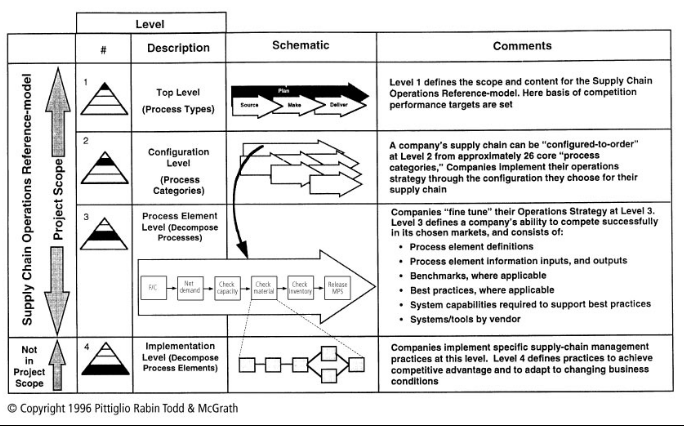
\includegraphics[width=.9\textwidth]{images/Stewart-1997.png}\\
  The four level model of SCOR as displayed in \cite{Stewart1997}
\end{center}

SCOR features four levels of supply-chain management:
\begin{itemize}
\item \textbf{Level 1} provides a broad definition of the plan, source, make,
  deliver process types, and is the point at which a company establishes its
  supply-chain competitive objectives.
\item \textbf{Level 2} defines 26 \emph{core process categories} that are
  possible components of a supply chain. A company can configure both its
  actual and ideal supply chain by selecting from these core processes.
\item \textbf{Level 3} provides a company with the information it needs to
  plan and set goals successfully for its supply-chain improvements through
  detailed process element information for each level 2 category. Planning
  elements include process element definitions, diagnostic metrics,
  benchmarks, best practices, and system software capabilities to enable best
  practices.
\item \textbf{Level 4} focuses on implementation, when companies put specific
  supply-chain improvements into play. Since changes at level 4 are unique to
  each company, the specific elements of the level are not defined within the
  industry-standard model.
\end{itemize}

SCOR focuses on four basic supply-chain processes:
\begin{itemize}
\item[(1)] \textbf{Plan:}
  \begin{itemize}
  \item \emph{Demand/supply planning:} Assess supply resources; aggregate and
    prioritize demand requirements; conduct inventory planning; assess
    distribution requirements; determine production, material, and rough-cut
    capacity for all products and all channels.
  \item \emph{Plan infrastructure:} Make/buy decisions; supply-chain
    configuration; long-term capacity and resource planning; business
    planning; product phase-in/phase-out; manufacturing ramp-up; end-of-life
    management; product line management.
  \end{itemize}
\item[(2)] \textbf{Source:}
  \begin{itemize}
  \item \emph{Sourcing/material acquisition:} Obtain, receive, inspect, hold
    and issue material.
  \item \emph{Source infrastructure:} Vendor certification and feedback;
    sourcing quality; inbound freight; component engineering; vendor
    contracts; initiation of vendor payment.  
  \end{itemize}
\item[(3)] \textbf{Make:}
  \begin{itemize}
  \item \emph{Production execution:} Request and receive material; manufacture
    and test product; package; hold and/or release product.
  \item \emph{Make infrastructure:} Engineering changes; facilities and
    equipment; production status; production quality; shop
    scheduling/sequencing; short-term capacity.
  \end{itemize}
\item[(4)] \textbf{Deliver:}
  \begin{itemize}
  \item \emph{Demand management:} Conduct forecasting; plan promotions; plan
    projects; plan sales campaigns; collect and analyse point of sale (POS)
    data and actual customer orders; promote products; price products; measure
    customer satisfaction; execute efficient customer response (ECR).
  \item \emph{Order management:} Enter and maintain orders; generate
    quotations; configure product; create and maintain customer database;
    manage allocations; maintain product/price database; manage accounts
    receivables, credits, collections and invoicing.
  \item \emph{Warehouse management:} Receive and stock finished goods; pick
    and pack; configure products; ship products; create customer specific
    package labelling; consolidate orders.
  \item \emph{Transportation management:} Manage traffic; manage freight;
    manage prod-uct import/export.
  \item \emph{Installation management:} Schedule installation activities;
    perform installation; verify performance.
  \item \emph{Deliver infrastructure:} Channel business rules; order rules;
    management of deliver inventories; management of deliver quantity.
  \end{itemize}
\end{itemize}

\section{Business Process Landscaping}

In contrast to \cite{FordMouzas2013} (see below), the significance of
\emph{Business Process Landscapes} (BPL) or -- better as verb --
\emph{Landscaping} is not primarily in the representation of cross-company
Process Landscapes as a generalisation of supply chain structures, but rather
in the company-internal shaping of Business Process descriptions.

BPL is thus part of a systemic double relationship of shaping cross-company
description structures of practices on the one hand (BPMN, APQC-PCF) and
implementing such description structures in the special company on the other.
The first process of cross-company standardisation unfolds as a \emph{systemic
  development process} on the background of the -- time-delayed -- unfolding
of \emph{process instances} of the second kind as systemic development
processes at company level.

This phenomenon of further development of a class itself in the course of its
repeated instantiations, unknown from (classical) OO programming, is an
essential phenomenon of the co-development of systemic structures at different
levels of abstraction. It plays a role in particular in the TRIZ construction
of the \emph{System Operator}, which relates the developments of the
supersystem and the system, although is not addressed that there is a
\emph{multitude} of systems related to a supersystem since the considerations
are centered at the (given) system.

It was not clearly explained in the presentation and discussion what is the
connection between the development of uniform \emph{structural} concepts at
the supersystem level and the diversity of \emph{procedural} applications in
the individual BPL instances. We mentioned earlier that in the APQC-PCF, from
the process level downwards, \emph{variations} allow to adapt the standard to
company-specific conditions, which results in a direct correlation between the
mapping of the APQC-PCF structures and the BPL practices in the respective
company.

The reverse conditionality -- the influence of experienced BPL practices on
those cross-company standardisation processes -- remained completely out of
consideration, especially the importance of formalising and structuring
"experienced results" of a BP landscaping for the company-wide model
structures as a link between BPL practices and those standardisation
\emph{processes} that ultimately find their \emph{structural} expression in
standards such as the APQC-PCF.

\section{Schematisation in the Work of G.P. Shchedrovitsky}

In the previous seminars we studied concept formation processes in the context
of description of organisations in general and entrepreneurial organisations
in particular. These concept formation processes are part of the general
formation of systemic structures and are at the same time an essential
emergent \emph{product} of these formation processes, i.e. they can only be
understood and have effect in the context of the "assembled" system as a whole
and its operation.

We further found out that such conceptual systems mark an important moment of
systemic "reduction to essentials" and thus form the decisive difference
between (simple) immersive and (more complex) submersive systemic structures.

It has been less clear so far how such conceptualisation processes take place
in practice in the interplay between modelling and planning as "justified
expectations" and the "experienced results" of planned action on this basis.

With the AFQC-PCF, we studied an already firmly established cross-company
conceptual system. On the other hand, we observed in seminars in earlier
semesters that such conceptual systems emerge as standards from a large excess
of theoretical approaches in a lengthy process of consideration and agreement.

We had also found such diversity in the internal modelling of business
processes (BP), especially in the concept of BP landscaping. In contrast to
the "free conceptualisation" in the course of the standardisation of BPMN or
AFQC-PCF, the processes of enterprise-internal BP modelling take place in the
context of a supersystem in which various conceptual systems have already
established themselves as standards. Nevertheless, we have seen that a simple
adoption of these conceptual systems for corporate modelling is not possible,
but detailing and varying modifications and instantiations are required.

G.P. Shchedrovitsky has structured such concept formation processes from a
philosophical perspective in more detail and summarised it in the approach of
"schematisation". These theoretical considerations are at the centre of both
the Methodological School of Management as a training institution and the
Organisational Activity Games (OAG\footnote{Somewhere also ODI --
  \foreignlanguage{russian}{Организационно-деятельностные игры}.}) organised
by him from 1979 until the 1990s, which played a major role in the preparation
and transition from a centrally controlled state economy to more market-based
forms on the territory of the former Soviet Union.

The notion of \emph{schematisation} is central in Shchedrovitsky's concept of
managerial activity, which he develops from a complex understanding of
systemic relationships. The notion does not appear in the presentation or in
the handout of the seminar that ends with \cite[figure 1.2, p. 11]{MSM} and
thus misses all substantial point which are developen in \cite{MSM} in the
further text.

In \cite{MSM} schematisation is first introduced on p. 66 as follows
\begin{quote}  
  What is important is not so much where we sit and think or even how we
  think.  What is important (this is a crucial point) is what we take as the
  object of our analysis, and our actions when we start setting out our
  thoughts on the blackboard or the drawing board. The important thing is what
  schema we draw on our board, what we represent as our object, what the
  schema of it is. If we draw an organisational structure, then that will be
  the object of our action. If we draw the interface of group
  administrative-managerial structures, they will be the object of our
  analysis and later of our action. If we draw production lines, they will be
  the object of our action. Do you see my point?

  The actions of an organiser, leader and manager consist in applying specific
  schemata to reality. The object structure that results will depend on which
  schemata the individual applies.
\end{quote}
It is preceded by conceptual differentiation between
\begin{itemize}
\item Organisation, organisational work and form of the life of the collective
  (p. 25),
\item the system-object relationship (p. 30),
\item the difference between mental activity (Denktätigkeit) and pure thinking
  (p. 33),
\item the concept of practice of thinking (p. 52),
\item the connection between problem, problematisation and systems analysis
  (p. 63)
\end{itemize}
to finally arrive at the difference between roles and role occupations ("the
administrative-organisational structure of places", p. 64). This is unfolded
in two concepts of the notion system, from which "the art of schematisation"
(p. 101) is derived. In a next step the question is discussed how such
systemic planning ultimately translates into practical action (transition to
activity, implementation, processes as ways of reading schemata etc.).

Literature on OAG:
\begin{itemize}
\item Robert E. Howell, Irena G. Postalenko and Dmitri M. Rabkine: The
  Organizational-Activity Game as a Method of Collaborative Planning and
  Problem Solving in the Former Soviet Union.
  \url{https://www.fondgp.ru/old/lib/int/12.html}
\item E.N. Korneyeva: \foreignlanguage{russian}{Организационно-деятельностные
  или проблемно-деловые игры}\\ (Organisational-activity or problem-solving
  games). In: \foreignlanguage{russian}{Активные методы
    социально-психологического обучения} (Active methods of
  socio-psychological learning)
  \url{http://cito-web.yspu.org/link1/metod/met110/node26.html}
\item G.P. Shchedrovitsky (1983):
  \foreignlanguage{russian}{Организационно-деятельностная игра как новая форма
    организации коллективной мыследеятельности} (Organisational Activity Game
  as a new form of organisation of collective thought activity)
\end{itemize}

\section{Exploitative and Explorative Business Process Improvement Patterns}

The planned student presentation was cancelled at short notice, so the topic
had to be developed discursively on a quickly created presentation based on
\cite{Lindskog2018} and \cite{Rosemann2020}. At the beginning, the
\emph{status of the seminar objective} achieved so far was presented once
again and the terms BP Modelling, BP Landscaping, BP Execution, BP Management
and BP Improvement were demarcated from each other.

We already observed earlier that with APQC-PCF, for example, there exist
\emph{established conceptual systems} that \emph{can} be used for a real-world
structuring of the process landscape within a company and \emph{should} also
be used in order to achieve comparability with other companies. On the one
hand, such comparability is the basis for learning from the experiences of
others. In an advanced form, such a conceptual system is also the basis for a
more precise coordination of supply chain processes beyond company boundaries.

We are dealing with \emph{two systemic levels of abstraction} -- the systemic
structure of the processes in the company and a cross-company systemic
structure. The latter seems strangely unbounded at first, in contradiction to
our postulate of the necessity of contextualisation of a system. However, when
studying the APQC-PCF we observed that contextualisations on different levels
of abstraction play a role and that conceptual systems on a cross-industry
level as well as domain-specific conceptual systems for individual industries
are of importance. The latter have a more restricted context, but are
conceptually richer than the APQC-PCF at cross-industry level. Here, the
submersive character of the relation between the various "reductions to
essentials" of systems at different levels of abstraction becomes visible once
again.

This is particularly evident in the need to provide for a controlled variety
of concretisations for the practical implementation of general
conceptualisations in special enterprise modelling as tayloring as is built
into the APQC-PCF hierarchy starting from the level of processes.

We learned about \emph{BP Landscaping} on the one hand as an instrument for BP
modelling of processes in the company related to each other and on the other
hand as an instrument for role-specific communication of parts of such models
and thus coupling the model to the real-world company processes. The
importance of this instrument for the further development of the company as a
\emph{living organisation} in the sense of Shchedrovitsky became less evident.
This development is primarily driven by the comparison of the \emph{justified
  expectations} derived from the modelling with the \emph{experienced results}
derived from practice. Here, instruments of \emph{measuring} and
\emph{benchmarking} play a crucial role, to translate the experienced results
back into the language of the model.

However, it is only from such a development perspective that problems can be
identified and solved (Shchedrovitsky: "You can only manage something that is
in motion.", "A system without problems does not need to be managed."). Thus
the object of \emph{Business Process Management} (BPM) is determined as "the
body of methods, techniques, and tools to discover, analyze, redesign, execute
and monitor business processes" \cite{Lindskog2018}. In this context,
\emph{discover} and \emph{analyse} is directed at the identification of
problems, \emph{redesign} at the planning of changes initially in the model,
\emph{execute} and \emph{monitor} at the practical implementation of these
changes and the monitoring of this transformation process. For this cyclic
process, also referred to as the \emph{BPM lifecycle}, exists a greater
variety of conceptualisations in the literature, see the slides of the
presentation for some of them.

\emph{BP Improvement} (BPI) is a slight variation of the way to view on BPM.
While BPM focuses on \emph{resilience} and thus on conservative or conserving
goals, BPI is more concerned with looking at the \emph{increment} achieved in
the course of running through such a lifecycle.

According to \cite{Rosemann2020}, this is also the difference between
exploitative and explorative improvement. The former serves to eliminate
problems in the "regular" behaviour and thus stabilise the system in the
existing context. The latter serves to find ways to adapt the system to
(possibly drastically) changing external conditions. The strategies thus refer
to different development paths of external conditions. The field of
\emph{exploitative improvements} focuses on better internal adaptation to
stable external conditions and is clearly elaborated in the literature in more
detail. \emph{Explorative improvements} are gaining in importance as the pace
of digital change increases. Rosemann's focus on \emph{revenue resilience},
however, is highly unspecific with regard to the \emph{reasons} for such
change and focuses on the revenue collapse as a sign of a need for action. The
proposed process improvement patterns remain at this level and do not search
for possible technical changes as the cause of the observed misery, i.e. they
only treat the symptoms.

The discussion focused on the concept of \emph{patterns} as a triple of
problem, context and solution (Christopher Alexander), under which successful
improvement strategies can be clustered. The \emph{TRIZ patterns}, the
\emph{40 principles} or the \emph{76 standards}, are characterised by the fact
that the path from the problem to the solution is described and justified in
more detail at a suitable level of abstraction, whereas the process and
business model patterns are limited to the proposal of solutions.

\section{Sustainable Business Model Patterns and Anti-Patterns}

With the last topics in the seminar, the perspective shifts from
\emph{Business Processes} to \emph{Business Models}. While Business Process
Landscaping focuses more on the level of the design of \emph{operational}
management tasks, Business Models deal with questions of the \emph{strategic
  orientation} of the company in order to sustainably secure relevant capital
flows and thus the decisive \emph{throughput} required for a viable business
system.

In the presentation such a perspective was linked with the questions
\begin{itemize}
\item Who is the customer?
\item And what does the customer value?
\item How do we make money in the business?
\item How we can deliver value to customers at an appropriate cost?
\end{itemize}
In addition to the definition of strategic business areas, it is about
identifying and addressing \emph{solvent demand} as well as the
\emph{cost-benefit structures} in the company.

However, business models are only one topic in the field of strategic
corporate management. A second, equally important topic is the further
development of the production-technical basis as the material conditions which
restrict the number of possible business models that can be realised. The
development and expansion of these material conditions requires long-term
capital commitment. This includes the retention and qualification of personnel
who can fill the intended roles, as well as stable supply chain conditions.

This material \emph{aspect of the possible} is largely ignored in the
perspective of Business Models, which concentrates on finding suitable value
propositions, i.e. identification of (additonal) solvent demand structures
that could be addressed in the context of the \emph{given} production
conditions or can be tapped by \emph{slightly modifying} them. Similar to the
view on technical systems as variable bundles of technical functions (see
\cite{Graebe-dat}), the company's production system is understood as a
variable bundle of business processes whose degrees of variability can be used
to adapt the Business Model.

Like the patterns of technical TRIZ, BM patterns abstract from these specific
variabilities and claim that a modest number of \emph{abstract patterns} can
be identified which recur frequently in such tasks to design a transformation
of a Business Model as a system of value propositions.

In the presentation itself, the area was explored using the example of the
topic of \emph{sustainability} as a new component of value proposition to be
integrated into existing BM. With the anchoring of the topic in public
awareness, it increasingly plays a role as an (additional) value proposition.

Sustainability is altogether a difficult topic, as processes on different
temporal dimensions with partly contradictory challenges are intertwined here.
The increasing attention to ecological issues for the design of BM, which has
gained massive increase in importance in recent years, at least in Western
Europe, is embedded in a global political process that lasts already 50 years,
since the publication of the "Limits to Growth" in 1972. In this process,
challenges increasingly get public attention that result from the fact that
our current mode of production is undermining the human existence in the long
term. In the climate debate, these challenges are increasingly operationalised
at the monetary level, whether as a CO$_2$ tax or in the "Paris gap". Somewhat
more abstract statements such as "peak oil", which still dominated the
discussions 10 years ago, have stepped into the background. The 17 Sustainable
Development Goals (SDG) adopted by the UN, as new reference point of the
politicisation of the issue are of particular importance.

The operationalisation in Business Models is faced with the fundamental
contradiction that a \emph{crucial change} in the mode of production is
required, which cannot be based on even innovative BM based on the
\emph{existing organisation of production}. However, the two sides of the
contradiction operate on different time horizons and thus on different
systemic levels. The PESTLE approach (political, economical, social,
technological, legal, environmental) attempts to bring those long-term
challenges as TRIZ \emph{fields} into the modelling of shorter-term systemic
transformations of BM.

BM patterns that incorporate such phenomena are thus only at the beginning of
a consolidation in corresponding processes of experience. An overview of such
patterns was given in the presentation. The suggestions for additional value
propositions in such patterns refer to a wide range of new BM approaches that
have come up in the context of the digital transformation. It remains to be
seen under which contextual conditions these approaches really lead to
success.

In another talk Ralf Laue gave an introduction into the concepts of the
\emph{St. Gallen Business Model Navigator}.

\section{Service  Oriented Business Process Management}

As a last topic the IMP concepts presented in \cite{FordMouzas2013} on
Interactive Business Landscapes at an inter-company level were presented and
discussed.

In the previous seminars, strategic corporate planning (business model design)
was considered from the perspective of an individual company and its world
conceptualisation. However, these world conceptualisations are related to each
other by \emph{practical dependencies} between the execution of the individual
business models. These dependencies can in turn be conceptualised, leading to
\emph{systemic development processes at an inter-company level}.  This further
dimension of cooperative action is addressed in \cite{FordMouzas2013} taking
the perspective of a rigorous developmental approach, as is also the case with
our concept of Cooperative Action.

This research relates to the Industrial Marketing and Purchasing (IMP) Group,
which is  
\begin{quote}
  an informal, international network of hundreds of scholars who approach
  marketing, purchasing, innovation, technological development and management
  from an interactive perspective, in a B2B and a B2C context. The IMP Group's
  current work also includes research on public-private networks, policy, and
  science-technology-business issues. ... (from their Website
  \url{https://www.impgroup.org/about.php}, )
\end{quote}
As explained there, the IMP Group stands for three main features: 
\begin{itemize}
\item[(1)] a dynamic approach to economic exchange,
\item[(2)] empirically driven research on inter-organizational interactions,
  and
\item[(3)] an informal network of researchers forming a vibrant international
  community.
\end{itemize}
Firstly, the IMP Group represents a dynamic approach to economic exchange,
which means that emphasis is placed on the interaction processes taking place
within and between business actors forming business relationships over time.
...

Secondly, the IMP Group represents a research tradition that places emphasis
on empirically-based studies of how companies actually do business and of the
various effects emerging when businesses and other organizations interact.
Based on the assumption of interdependent business actors, a hallmark of IMP
studies is that marketing, purchasing, technological development, innovation,
strategic management and logistics need to be investigated \emph{within the
  context of specific business relationships and networks}.

Thirdly, the IMP Group represents a large informal network of researchers. The
IMP Conference and the IMP Journal Seminar are important meeting places for
researchers from all over the world, all sharing an interactive perspective on
the business landscape. ...

The following explanations are mainly taken from \cite{FordMouzas2013}.

IMP Conceptualisations are based on a notion of \emph{Business Processes}
which are conceptualised as \emph{substantive} interaction between
\emph{activities}, \emph{resources} and the \emph{actors} associated with
them.  The \emph{heterogeneity}, the importance of \emph{specific
  counterparts}, the \emph{complexity} and \emph{long-term nature} of business
interaction argue against generalisations about particular categories of
actors such as ‘customers’, ‘suppliers’, ‘manufacturers’ or ‘retailers’ to
conceptualise their interactions.

IMP research is concerned to examine the idiosyncratic \emph{Network Pictures}
held by the actors within their \emph{small world} of tight functional
dependencies which form the basis of their approaches to interaction.  Such
analysis suggests that the small world of the business actors does not exhibit
the characteristics of a \emph{market} nor is it simply an \emph{agglomeration
  of many markets}: Its structure is not one of independent companies that
have ease of entry or exit from the market or from their dealings with specific
counterparts as marketers or customers. Instead, the analysis emphasises that
many of the actors in this small world are strongly interdependent with each
other through their business.

The pattern of interdependencies across these small worlds and the
perspectives that arise from them form the \emph{context for continuing
  interaction} and the developments.  This small world is a \emph{cooperative
  action space} as developed in the lecture where "relational moments between
actors shape the cooperative context more than individual moments of
individual actors“ with narrow, but permeable boundaries.

Interactions in business are not restricted to communication, negotiation or
to specific transactions but are \emph{substantial} and \emph{material}. In
other words, they involve a number of different aspects of the (practical)
\emph{activities} and (material) \emph{resources} of the actors which may be
changed and transformed and hence \emph{evolve} during action.

In the paper an example is given: The development of ready-meals changes
aspects of the activities, resources and the actors involved in this small
world. Some activities such as the production systems of food producers
becomes more or less specialised towards the requirements of particular
counterparts.  Resources, such as the stockholding facilities of producers,
retailers and logistics companies will have followed a particular \emph{path
  of investment} or development and the actors themselves will have
\emph{co-evolved}.

Co-evolution does not refer to an inevitable increase in the ‘closeness’ of
the relationships between interacting actors. Rather, it suggests that
\emph{the operations, characteristics and attitudes of business actors evolve
  as an outcome of their interactions} over time and thus the set of
relationships evolves itself.  In this context Vargo and Lusch bring it to the
point: "Resources are not, they become".

All the actors are part of a \emph{wider network} of substantial practical
dependencies.  However, each of these actors has a very restricted picture of
this "wider world" and no direct interaction with most of the actors within
it.  For this reason, actors are dependent on \emph{service provision} by some
of its immediate counterparts who have relationships with or provide access to
others at a distance. Such service is similar to using \emph{components off
  the shelf} (COTS) in Component Software but in a production-organisational
and not in a technical perspective.

This leads to a view of interaction in business relationships as a unique,
evolving, multifaceted process of \emph{‘problem-coping’ by and for all of the
  involved actors} (Webster 1965). This relates to Shchedrovitsky's claim:
"If there are no problems, no management is required“.

The term ‘coping’ is used to emphasise the interactive and evolving nature of
business problems.  Such 'problem coping' by service-seeking and offering
drives the process of \emph{activity specialisation}, \emph{division of labour
  by specialisation}, the \emph{path of resources} and the \emph{co-evolution
  of actors}.

The most significant problems that actors face concern \emph{the relationship
  structure in which they are embedded}. The business actor should be viewed
as a \emph{node} within a network of relationships, so that what happens
outside the actor (i.e. inside its "small world") and through its
relationships is likely to be more important in the evolution of that actor
than what happens inside.  More important than the current structure of that
network is its development potential.  Hence IMP research uses the verb
\emph{business networking} to refer to the attempts of actors to change the
structure and process of the relationships in which they are involved.

It is through business networking that actors seek to cope with their problems
and those of others.  Costs of this problem coping by Business Networking can
be considered under the following aspects.
\begin{itemize}
\item Short-term, \emph{dyadic} problem coping may centre on a single
  transaction involving the costs associated with transferring cash for one
  counterpart and the benefits of service for the other (cost-benefit
  relation).
\item Short-term problem coping may involve working together to solve a
  particular technical problem for \emph{mutual benefit} (mutual benefit
  relation).
\item Short-term problem coping may appear to involve only one actor in
  benefits and one in only costs. However, these \emph{short-term costs and
    benefits} received will affect both actors \emph{long-term view} of their
  relationship.  The long-term view considers short-term costs as
  \emph{investment}.
\item In the longer term, problem coping will be based on such
  \emph{investments} and \emph{adaptations} by the counterparts (\emph{synergy
    effects}) in one or more aspects of the substance of their interaction.
\end{itemize}
Business actors commonly face issues over the \emph{trade-offs between
  potential and actual short-term and long-term costs and benefits} of the
counterparts in relationships, expressed in terms of the \emph{extent and
  timing} of respective activity specialisation, resource path or actor
co-evolution.

It is likely that actors would perceive that much of the service actually
provided fell short of their expectations or exceeded them.  \emph{Unforeseen
  contingencies} might explain this: late delivery of services or products,
not forthcoming cooperation, only partial adaptations, payment less than
expected etc. In contrast, technical assistance could produce greater than
anticipated cost savings or a cooperative development could enhance an actor's
relationship with a third party.

The existence of different perceptions among actors explains why profitable
business opportunities may exist whenever \emph{prices fail to reflect the
  value}.  The value to a participant from service is not a characteristic of
what is involved in it, whether product, services, payment or generalised
‘performance’.

An interactive and systemic conceptualisation of the business process requires
a refinement of this view of value in different directions.
\begin{itemize}
\item \emph{Value of problem coping:} As problem-coping process the value to
  each actor of a service is that \emph{actor's interpretation} of the worth
  of the service's contribution towards coping with one or more specific
  problems of the actor, \emph{identified by that actor}.

  Hence the value as the ‘perceived worth’ of the same service received by
  different respondents will be different and in all cases that value is time
  and problem-specific.

  Empirically, this nature of service value to a counterpart poses great
  difficulty for the provider in business interaction.

\item \emph{Value and reciprocity:} The value of service is not determined
  solely by the receiving actor but also assessed by the service supplier.
  Each party makes its own assessment of the problem-specific value to
  themselves and to their counterparts of a service that they seek or provide.

  These multiple assessments form the basis for their approach to interaction
  in any single episode and to their expectations and intentions for future
  episodes and a relationship as a whole.

\item \emph{Incidental value:} The business landscape is characterised by
  recurrent interactions between multiple actors in continuing relationships.

  Service provision and value creation in any of these may lead to incidental
  value to others, either positive or negative and in line or against the
  wishes of those involved.
\end{itemize}

The concept proposed in \cite{FordMouzas2013} connects
\begin{itemize}
\item \emph{Business interaction} as problem-coping process of actions,
  reactions and re-reactions between actors,
\item \emph{Services} as suuccessive outcomes of business interactions as
  perceived by the participants and
\item \emph{Value} as actor's perception of the contribution of service to
  coping with a specific or general problem of particular actors.
\end{itemize}

Value of service may be identified at the following levels:
\begin{itemize}
\item \emph{Episodic service value:} Service provision within a particular
  interaction episode. Value creation is the outcome of solving a particular
  problem rather than to conform to current ways of operating.

\item \emph{Relational service value:} Continuing or long-term service
  interaction in a dyadic relationship by developing the potential value of
  the relationship for future episodes.  Relational value at any one time
  depends on the interdependence of the counterpart's activities, the
  heterogeneity of their resources and the jointness of the actors.

\item \emph{Service value in the small world:} Network effects for actors
  when to consolidate interactions within existing relationships, to change
  their pattern or to develop new relationships.

  The costs and time involved in new relationship development often limit
  networking opportunities to existing relationships.

  However, problem coping in the business landscape \emph{can never be wholly
    dyadic}.  The service offered by a single actor to another always depends
  on service provision from other relationships.  An obvious example of this
  is seen in the dependence of product suppliers on components supplied by
  others.

\item \emph{Service value in the wider world:} Because of an actor's lack of
  knowledge or established relationships in the wider world, this networking
  will either be based on \emph{relationship development} or \emph{service
    provision} by others.
\end{itemize}

\cite{} draw the following conclusions.
\begin{enumerate}
\item The conceptualisation of service in an interactive business landscape
  allows to capture the inherent connectivity among interdependent business
  actors.

  This connectivity leads to a view of service as the successive and
  reciprocal outcomes of recurrent interaction between multiple actors as
  perceived by the involved business actors.

\item The idea of service in an interactive business landscape transforms our
  view of the process of value creation and appropriation in networks.

  The value of a service is not confined to the provision by one company
  (supplier) to an apparent receiver (customer).  Instead, service in the
  business landscape is a \emph{systemic process} producing different positive
  and negative value for multiple actors, including those that appear only to
  be providers.
  
  The value of service is not confined to a single episode in which service
  appears to have been provided.

  A particular interaction episode that provides immediate value is also
  likely to change the nature of the relationship in which it occurs, leading
  to relationship value.

\item Taking an interactive approach to service allows to investigate the
  \emph{dynamics} of problem coping and creation.

  The evolution of problem-coping is observable through a continuing cycle of
  recurring episodes and evaluations over time ("justified expectations" and
  "experienced results" in the terminology of the lecture).

  For the management, the idea of service in an interactive business landscape
  emphasises the importance of \emph{analysing} the evolving problems and
  uncertainties of specific actors and the perceptions of those involved in the
  interaction.
\end{enumerate}

The concept of service highlights interaction in continuing relationships as
the successive, reciprocal, outcomes of action, reaction and re-reaction of
counterparts and thus the \emph{evolution of the "small world"}.  This
requires perceptive analysis of relationship evolution, of the problems of the
company and its counterparts and a well developed, explicit but flexible
agenda.

Service in an interactive business landscape also involves a \emph{managerial
  reorientation} away from things, products and services and towards the
evolving problems of the company and its specific counterparts.

\emph{Service provision} can range from obvious manifestations, such as the
payment of an invoice, the delivery of a product or the development of a new
technology to the subtle or complex, including the provision of advice or
reassurance, organisational transformation or intellectual assets, know-how
and expertise.

The nature of service delivery is \emph{defined by the recipient} and its value
is determined by the problems of the recipient.

An understanding of the concept of service and value in an interactive
business landscape enables managers to \emph{relate their own resources and
  activities} to those of others as the basis of coping with their respective
problems ("The whole is more than the sum of its parts").

\raggedright
\begin{thebibliography}{xxx}
\bibitem{Ackoff1997} Russell L. Ackoff (1971). Towards a system of systems
  concept.  Management Science 17 (11), 661-671.
\bibitem{APQC-PCF} The APQC Cross Industry Process Classification Framework.
  Version 7.2.1, Sept. 2018.
\bibitem{Bolstorff2017} Peter A. Bolstorff (2017).  20 Years of SCOR:
  Reflections on Relevancy and the Road Ahead. ASCM Blog, 03/27/2017.
  \url{https://www.ascm.org/}
\bibitem{foaf} FOAF Vocabulary Specification (2014). W3C Recommendation.
  \url{http://xmlns.com/foaf/spec/}.
\bibitem{FordMouzas2013} David Ford, Stefanos Mouzas (2013). Service and value
  in the interactive business landscape. Industrial Marketing Management 42,
  9–17.  \url{http://dx.doi.org/10.1016/j.indmarman.2012.11.003}
\bibitem{Graebe-mts} Hans-Gert Gräbe (2020). Men and their technical systems
  (in German).\\ LIFIS Online, 19 May 2020.
  \url{https://doi.org/10.14625/graebe_20200519}.

  A shorter English version is available at
  \url{https://hg-graebe.de/EigeneTexte/sys-20-en.pdf}
\bibitem{GraebeKleemann} Hans-Gert Gräbe, Ken Pierre Kleemann (2020). Seminar
  Systemtheorie. Universität Leipzig. Wintersemester 2019/20 (in German).
  Rohrbacher Manuskripte, Heft 22. LIFIS Berlin.
\bibitem{Graebe-dat} Hans-Gert Gräbe (2021). Technical Systems and Their
  Purposes. In: O. Mayer (ed.) TRIZ-Anwendertag 2020. Springer.
  \url{http://dx.doi.org/10.1007/978-3-662-63073-0_1}.
\bibitem{Haertel2021} Stefan Härtel (2021). Slides to his talk on November 16,
  2021.  Available in the github repo.
\bibitem{Lindskog2018} Carin Lindskog (2018). Exploitation and Exploration in
  Business Process Management – An exploratory paper. CEUR Workshop
  Proceedings, pp. 405-414.
\bibitem{vocab-org} The Organization Ontology (2014). W3C Recommendation.
  \url{https://www.w3.org/TR/vocab-org}.
\bibitem{Petrov2020} Vladimir Petrov (2020). Laws and patterns of systems
  development (in Russian). ISBN 978-5-0051-5728-7.
\bibitem{Rosemann2020} Michael Rosemann (2020). Explorative process design
  patterns. In: Fahland, Ghidini, Becker, Dumas (Eds.). Business Process
  Management: 18th International Conference, BPM 2020 Proceedings,
  pp. 349-367. \url{https://eprints.qut.edu.au/201691/}
\bibitem{MSM} Georgy P. Shchedrovitsky. Selected Works. Part I in Viktor
  B. Khristenko, Andrei G. Reus, Alexander P. Zinchenko et al. (2014).
  Methodological School of Management. Bloomsbury Publishing.  ISBN
  978-1-4729-1029-5.
\bibitem{Sommerville2015} Ian Sommerville (2015). Software Engineering.
  Chapter 19 „Systems Engineering“.
\bibitem{Souchkov2010} Valeri Souchkov (2010). TRIZ and Systematic Business
  Model Innovation.  In: Proceedings TRIZ Future Conference 2010, Bergamo,
  Italy.
\bibitem{Souchkov2014} Valeri Souchkov (2014). Breakthrough Thinking with TRIZ
  for Business and Management: An Overview.
  \url{http://www.xtriz.com/TRIZforBusinessAndManagement.pdf}
\bibitem{Souchkov2017} Valeri Souchkov (2017). Accelerate Innovation with
  TRIZ.
  \url{http://www.xtriz.com/publications/AccelerateInnovationWithTRIZ.pdf}
\bibitem{Souchkov2019} Valeri Souchkov (2019).  TRIZ for Business and
  Management: State of the Art.  TRIZ Developers Summit 2019.
\bibitem{Stewart1997} Gordon Stewart (1997). Supply-chain operations reference
  model (SCOR): the first cross-industry framework for integrated supply-chain
  management. Logistics Information Management, vol. 10 (2), pp. 62–67.
\bibitem{Szyperski2002} Clemens Szyperski (2002). Component Software. Pearson
  Education.  2. Auf\-lage.  ISBN 0201745720.
\bibitem{TOP} The TRIZ Ontology Project.
  \url{https://wumm-project.github.io/Ontology.html}.
\end{thebibliography}

\end{document}
